\documentclass[12pt,abstract=true]{scrartcl}

%<<< Preamble
\usepackage{tikz}
\usepackage{array}
\usepackage{pifont}
\usepackage{engord}
\usepackage{listings}
\usepackage{titlesec}
\usepackage{fancyhdr}
\usepackage{fancyvrb}
\usepackage{multicol}
\usepackage{pgfplots}
\usepackage{algorithm}
\usepackage{algpseudocode}
\usepackage[plain]{fancyref}
\usepackage[unicode]{hyperref}
\usepackage{graphicx,tabularx}
\usepackage[shortlabels]{enumitem}
\usepackage[retainorgcmds]{IEEEtrantools}
\usepackage{amsmath,amssymb,amsthm,amscd,amstext}
\usepackage{mathtools}
\usepackage{exscale}
\usepackage{relsize}
\usepackage{mathrsfs}
\usepackage{tocloft}

\usepackage{setspace}
\usepackage{lastpage}
\usepackage{extramarks}
\usepackage{chngpage}

\usepackage{lmodern}
\usepackage{mathpazo}

%\pgfplotsset{compat=1.6}
\usetikzlibrary{arrows}
\usetikzlibrary{patterns}
\usetikzlibrary{positioning}
\usetikzlibrary{automata}
\usetikzlibrary{plotmarks}
\usepackage{tikz-3dplot}

\tikzset{ alert/.style={ very thick, draw=red!80, fill=red!20 } }
\tikzset{ fancy/.style={ very thick, draw=blue!80, fill=blue!20 } }
\tikzset{
  dot/.style={
    very thick,circle,draw=black,fill=black,inner sep=0,minimum size=5pt
  }
}
\tikzset { every state/.style={fancy} }
\tikzset {
  general/.style = {
    shorten >=2pt, node distance=2.5cm, on grid, thick,>=stealth', auto
  }
}
\newcommand{\mathhuge}[1]{\mathlarger{\mathlarger{\mathlarger{#1}}}}
\newcommand{\mathtiny}[1]{\mathsmaller{\mathlarger{\mathlarger{#1}}}}

\renewcommand\cftsecfont{\normalsize}
\renewcommand\cftsecpagefont{\normalsize}
\renewcommand\cftsecafterpnum{\par}
\setlength{\cftbeforesecskip}{0.2em}

\renewcommand\cftsubsecfont{\small}
\renewcommand\cftsubsecpagefont{\small}
\renewcommand\cftsubsecafterpnum{\par}

\newcommand\upper[1]{\textsuperscript#1}
\numberwithin{equation}{section}
\mathtoolsset{centercolon}
\bibliographystyle{plain}

% Theorem environment <<<
\theoremstyle{definition}   \newtheorem{definition}{Definition}[section]
\theoremstyle{plain}        \newtheorem{theorem}{Theorem}[section]
\theoremstyle{plain}        \newtheorem{observation}{Observation}[section]
\theoremstyle{plain}        \newtheorem{fact}{Fact}[section]
\theoremstyle{plain}        \newtheorem{claim}{Claim}[section]
\theoremstyle{plain}        \newtheorem{lemma}[theorem]{Lemma}
\theoremstyle{plain}        \newtheorem{corollary}[theorem]{Corollary}
\theoremstyle{remark}       \newtheorem{example}{Example}[section]
\theoremstyle{remark}       \newtheorem{remark}{Remark}[section]
\newcommand*{\fancyrefdeflabelprefix}{def}
\newcommand*{\fancyrefthmlabelprefix}{thm}
\newcommand*{\fancyreflemlabelprefix}{lem}
\newcommand*{\fancyrefcorlabelprefix}{cor}
\newcommand*{\fancyrefalglabelprefix}{alg}
\newcommand*{\fancyreflnlabelprefix}{ln}
\frefformat{plain}{\fancyreflnlabelprefix}{line #1}
\Frefformat{plain}{\fancyreflnlabelprefix}{Line #1}
\frefformat{plain}{\fancyrefalglabelprefix}{algorithm (#1)}
\Frefformat{plain}{\fancyrefalglabelprefix}{Algorithm (#1)}
\frefformat{plain}{\fancyrefdeflabelprefix}{definition (#1)}
\Frefformat{plain}{\fancyrefdeflabelprefix}{Definition (#1)}
\frefformat{plain}{\fancyrefthmlabelprefix}{theorem (#1)}
\Frefformat{plain}{\fancyrefthmlabelprefix}{Theorem (#1)}
\frefformat{plain}{\fancyreflemlabelprefix}{lemma (#1)}
\Frefformat{plain}{\fancyreflemlabelprefix}{Lemma (#1)}
\frefformat{plain}{\fancyrefcorlabelprefix}{corollary (#1)}
\Frefformat{plain}{\fancyrefcorlabelprefix}{Corollary (#1)}
%>>>
% Alter some LaTeX Float for better treatment of figures: <<<
% See p.105 of "TeX Unbound" for suggested values.
% See pp. 199-200 of Lamport's "LaTeX" book for details.
%   General parameters, for ALL pages:
\renewcommand{\topfraction}{0.9}	% max fraction of floats at top
\renewcommand{\bottomfraction}{0.8}	% max fraction of floats at bottom
\setcounter{topnumber}{2}
\setcounter{bottomnumber}{2}
\setcounter{totalnumber}{4}     % 2 may work better
\setcounter{dbltopnumber}{2}    % for 2-column pages
\renewcommand{\dbltopfraction}{0.9}	% fit big float above 2-col. text
\renewcommand{\textfraction}{0.07}	% allow minimal text w. figs
\renewcommand{\floatpagefraction}{0.7}	% require fuller float pages
\renewcommand{\dblfloatpagefraction}{0.7}	% require fuller float pages

\allowdisplaybreaks[4]

%>>>
%>>>

\begin{document}

\begin{center} %<<< Title
	\Large \textbf{\textsf{
		Metrics and Algorithms for Evolving Social Networks}} \\[2em]
	\normalsize 
		Pufan He\upper{1}, Yichao Zhou\upper{2}, Qiwei Feng\upper{3},
		Yu Yan\upper{4}, Qingyang Li\upper{5} and Xin
		Xing\upper{6}\\[1.5em]
	\small
	\begin{tabular}{*{3}{>{\centering}p{.3\textwidth}}}
		\upper{1}\small\href{mailto:hpfdf@126.com}{hpfdf@126.com} &%
		\upper{2}\href{mailto:broken.zhou@gmail.com}{broken.zhou@gmail.com} &%
		\upper{3}\href{mailto:gdfqw93@163.com}{gdfqw93@163.com} \tabularnewline
		\upper{4}\href{mailto:whyvine@hotmail.com}{whyvine@hotmail.com} &
		\upper{5}\href{mailto:591527324@qq.com}{591527324@qq.com} &
		\upper{6}\href{mailto:823291634@qq.com}{823291634@qq.com}
	\end{tabular} \\[1.5em]

	\small Institute for Interdisciplinary Information Sciences,
	Tsinghua University \\[2em]
	\normalsize
\end{center} \par %>>>

\begin{abstract}
This article addresses the dynamic properties of typical social networks. By
supposing that the evolution over time only includes creating new edges but no
deletion, we studies the activity and centrality metrics for nodes in
such graphs by regulating a series of reasonable properties the metrics should
satisfy. Then formal definitions are given to our metrics and
their mathematical analysis are put. We have developed a practice based framework
to maintain the evolving large-scale network and an algorithm to compute our
metrics including historical queries in acceptable time and space consumption.
Finally, we use a simple model to generate evolving graph from existing social
network data and compare our metric to the static one. The results imply
that dynamic centrality is more capable in spotting hot social events.

\smallskip
\noindent \textbf{Keywords:} social network, dynamic graph, vertex activity,
centrality, online algorithm.
\end{abstract}
% \tableofcontents
\newpage

\section{Introduction}
Social networks is a surprising interdisciplinary field of social science and
computer science, allowing helpful analysis of large-scaled social behavior
and tendency. In this article, we are able to deal with more information, the
time dimension, of social networks, and make a similar study to the social
behaviors.  We build metrics for evolving social networks and design an
algorithm to calculate them. We compare out results with the classical analysis
which works under un-timestamped data.

\subsection{Dynamic Metrics}
Networks contain too much information to be easily observed by people without
any abstraction. To study a network, people exploit the basic form of
quantification to concentrate on specific features of the whole graph or an
individual vertex. Our work is to extend this method to the dynamic graphs. We
basically design new dynamic metrics according to existing successful static
ones, but we will point out a important metric that can be only observed in
time evolving networks, the activity. Intuitively speaking, a vertex with high
activity indicates more frequent recent social actions, and the vertex is more
willing to make new change by the structural sense of graph. The accuracy of
activity will be quite vital to recommendation algorithms of advertisement, new
friends, or search results. Activity can be also used by other metrics, so that
the computation of other metrics will no longer need the time information
directly, but refer to the activity instead.

Centrality, usually defined on vertices, is frequently used to measure the
importance of a specific node in graphs of all kinds. There are many previous
studies about the static graph centralities\cite{newman2010networks}, such as
PageRank algorithm\cite{page1999pagerank}, and there are many useful network
analysis algorithms that used some forms of graph centralities. However, most
social networks change over time, and even more unfortunately, many of the
networks are large-scaled, which could make the analysis become hard and
costly, hence limiting the scale of meaningful data mining. Moreover, the time
effect can also become a factor of the centrality, that is, the same graph with
different evolving sequence may have totally different metrics. On an intuitive
level, the node connected with more higher activity nodes should be more
important at that time, even if other node have much more silent neighbors. If
we do not excavate the information on the time dimension, we will lose
tremendous information and also the possibility of accumulative computation
which could be helpful in enhancing the speed of answering consistent
querying.

In section 3 we will concentrate on centrality and activity in evolving social
network. We will define what kind of activity is good, and we will design
an instance of those metrics by the standard we set. In section 4, we will
give the algorithms to compute our designed centrality and activity from the
online data structure which maintains the evolving social network. We will also
show how to quickly locate significant vertices that has high activity or
centrality at a specific time. In section 5, we will show the metrics make
sense with real world data.

\subsection{Algorithms}
Graph theory is very successful on storing and solving various problems on
static networks. We have sophisticated method on finding the shortest
paths, getting a minimal spanning tree, finding the maximal $S$-$T$ flow, etc.
And we also have a well-established theoretical system to study problems that
do not seems to have perfect solutions. However, dynamic queries can be
very hard for general graphs. Best known solutions for many dynamic basic graph
problems still remain unsatisfiable for general demands. So to design metrics
for a general evolving network is a challenging and open problem. We
concentrate on the popularly studied social networks and try to create meaningful
and available approaches of operations on such networks.

In section 2, we will discuss the known properties of a typical social network,
which could be helpful for our algorithm designs. In section 4, we will
establish a framework of data structure and algorithms to solve series of
possible queries including computing the metrics about an evolving social
network.

\section{Evolving Social Network}
In some related research on evolving graphs, the time dimension is represented
by constructing a sequence of graphs $\{G_t(V_t,E_t)\}$ on different time
spots $t$. This model is highly expressive and universal in mathematical
statement, thus we adopt in. However, we constrain the relation of
time-adjacent graphs in order to simplify the analysis and remain the highest
possible loyalty to the real data generation. We build the \textbf{pure growing
model}, which cares about the new connection forming among vertices, neglecting
the anti-growing operations such as edge deletions. We assume the existence of
every connection will contribute to the metrics, even if the connection is
later erased. So we do not delete edges or nodes in our model, instead we could
add an decay mechanism to reduce the affect of old formed links, which will be
discussed in the next section. In pure growing model, we will assign every edge
a timestamp, namely what time the edge is created. Thus there could be more
than one edges between a pair of nodes with different timestamps.

\subsection{Definition}
\begin{definition}
A \textbf{pure growing model} for an evolving graph $G$ is defined in pair:
\begin{equation}
G=(V,E),
\end{equation}
where $V$ is the set of all nodes in the network, and $E$ is the set of edges.
For every $(u,v,t)\in E$, where $u,v\in V$ are the two end
points of the edge, ($u<v$ in case of bidirectional graph),
$t\in \mathbb{N}$. The $t$
component stores the forming time of the edge. As for weighted evolving graph
model, we modifies $e\in E$ for $e=(u,v,t,w)$, where $w\in\mathbb{R}^+$ stands
for the multiplicity of the edge, which might be useful in some circumstances,
and the others stay the same meaning. In the unweighted case, we can simply set
$w=1$ for all edges.
\end{definition}

\begin{definition}
The historical edge set $E_t$
\begin{equation}
E_t=\{e\;|\;e(u,v,t',w)\in E\text{ and }t'\leq t\}.
\end{equation}
An immediate statement one can ensure is
\begin{equation}
\forall t: E_t\subseteq E\text{ and }p\leq q\implies E_p\subseteq E_q.
\end{equation}

Define $G_t$ to be the graph formed by $V$ and $E_t$. So $G_t$ is the snapshot
of the whole network at time $t$.
\end{definition}

Now we define the update of an evolving graph in our model. First we assume all
possible active vertices has been already defined, so $V$ does not change.

\begin{definition}
$G^*(V,E^*)$ is the updated version of $G$, where $E\subseteq E^*$. We assume
the edges are added to the
model by correct time order, namely
\begin{equation}
\forall (u,v,t,w) \in E^*\setminus E,\, \forall (u',v',t',w')\in E: t \geq t'.
\end{equation}
\end{definition}

And we define the notation of some frequently used basic functions:
\begin{definition}
The adjacency matrix
\begin{equation}
A(G_t)=\begin{pmatrix}a_{ij}\end{pmatrix}_{n\times n},\text{ where }n=|V|,
a_{ij}\in \mathbb{R}^+,
\end{equation}
is the adjacency matrix of the graph at time $t$. More detailed
\begin{equation}
a_{ij}=\begin{cases}
0&(i=j)\\
\sum_{(i,j,t',w)\in E_t}w &(i<j)\\
a_{ji}&(i>j)
\end{cases}.
\end{equation}
Or, in case of directional graph,
\begin{equation}
a_{ij}=\begin{cases}
0&(i=j)\\
\sum_{(i,j,t',w)\in E_t}w &(i\neq j)
\end{cases}
\end{equation}
\end{definition}

\begin{definition}
The degree function $k(G_t,v)$.
\begin{equation}
k(G_t,v)=\sum_{\mathclap{(x,y,t',w)\in E_t}}(1-\delta(x,v)\delta(y,v))w,
\end{equation}
where \begin{equation}
\delta(x,y)=\begin{cases}1&(x\neq y)\\0&(x=y)\end{cases}.
\end{equation}
\end{definition}

\subsection{Properties}
In most social networks, people have their own friendship circles, and the
average circle size is quite limited because people do less interaction with
strangers than their close friends or family members. We call this phenomenon
the \textbf{sparsity} of social network.

\begin{definition}
Reduced edge set (historical) $E_t^\bullet=\{(x_i,y_i)\}$:
\begin{equation}
(x,y)\in E_t^\bullet \iff \exists e: e=(x,y,t,w)\in E_t.
\end{equation}
\end{definition}

\begin{definition}
Reduced degree $k^\bullet(G_t,v)$:
\begin{equation}
k^\bullet(G_t,v)=\Big|\{u\;|\;(u,v)\in E_t^\bullet\text{ or }(v,u)\in
E_t^\bullet\}\Big|.
\end{equation}
\end{definition}

We then have
\begin{equation}
\left<k^\bullet\right>=2\left|E^\bullet\right|/\left|V\right|,
\end{equation}
where $\left|E^\bullet\right|/\left|V\right|$ only depends on the structure of
the network at a time spot. In many available online datasets,
we can assume $\left<k^\bullet\right>$ is limited by a constant $K$, typically
$10^2$.
\definition Sparcity constant $K=\left<k^\bullet\right>$.

\begin{observation} $K=O(1)$.
\end{observation}
So if we only use the reduced edge list in our framework as additional memory
requirements, namely considering the adjacency matrix to be a sparse matrix and
only store the non-zero entries, the space expense would then be just $O(n)$,
which is highly available. However this does not means we can handle neighbor
updating operations in $O(1)$ time, because
\begin{equation}
\max k^\bullet\geq \left<k^\bullet\right>=K
\end{equation}
and the former one may be very large.  We cannot trivially assert the amortized
time complexity to be $O(1)$ neither, because the nodes with high degrees may
requires more operations over time, just like the famous friendship
paradox\cite{feld1991your}.

Another famous property of social networks is known as the small world
effect\cite{buchanan2003nexus}, for that the giant component contains nearly
all active nodes and it has very small diameter.

The clustering coefficient\cite{newman2010networks}, namely
\begin{equation}
c.c=\frac{\#\text{closed paths of length 2}}{\#\text{paths of length 2}},
\end{equation}
for a typical social network is a positive number, which means people are more
willing to make interactions with close related people than unfamiliar ones. 

\section{Activity and Centrality}

\subsection{Desiderata}
\definition $\mathit{Act}(G_t,v)$ returns the activity of node $v$ in the evolving graph in
time $t$. Then $\mathit{Act}(G_t,v)$ should be a deterministic function of $v$ and
$E_t$.
\begin{itemize}
\item \textbf{normalization}:

We want the metrics to derive other functions, so it will be nice if we can
limit the range of the function:
\begin{equation}
0\leq \mathit{Act}(G_t,v) \leq 1.
\end{equation}

\item \textbf{initialization}:

A node with no neighbors is totally inactive:
\begin{equation}
k(G_t,v)=0\implies \mathit{Act}(G_t,v)=0.
\end{equation}
Also we declare that
\begin{equation}
k(G_{-\infty},v)=0.
\end{equation}

\item \textbf{monotonicity}:

If a vertex $v$ performs an interaction $(v,u)$ at time $t$, i.e., a new edge
is added to $G_t$, and the interaction is the only change to the graph
at time $t$, then the activity of $v$ should be greater than if the edge is not
added.
\begin{equation}
E_t=E'_t\cup\{e(u,v,t,w)\}\implies \mathit{Act}(G_{t},v)>\mathit{Act}(G'_{t},v
).\label{eq-mono}
\end{equation}

\item \textbf{symmetry}:

For a node $v$ who created new connections at time $t$, we do not care about
the connection's target nor how is $v$ like before the connection, so
maintaining the change of $\mathit{Act}$ only depends on its current
$\mathit{Act}$ value and the $w$ values in the new edges. This property makes
activity a fair metric for all vertices, and also simplifies the computation.

There exists a function $g$, such that for any possible change
$E_{t+1}=E_t\cup\{e_i(u_i$, $v_i$, $t+1$, $w_i)\}|_{i=1}^n$,

\begin{equation}
\mathit{Act}(G_{t+\varepsilon},v)=g(\mathit{Act}(G_t,v),n,\{w_i\},\varepsilon),
\label{eq-sym}
\end{equation}
where $0<\varepsilon<2$.

\item \textbf{locality}:

We make activity the own property of a single node, so the actions in the
network in which the node did not participate will not affect the metric.

\begin{equation}
p<q\text{ and }k(G_p,v)=k(G_q,v)\implies \mathit{Act}(G_q,v)=\mathit{Act}(G'_q,v),\label{eq-loc}
\end{equation}
where $G'_q$ has exactly the same structure of $G_p$, excepting for the time
shift from $p$ to $q$.

\item \textbf{integrity}:

The quantity of actions for a node over time is a discrete function, so we
cannot define its derivation $f(t,v)=\frac{\mathrm{d}}{\mathrm{d}t}k(G_t,v)$
directly. However, we reverse this property, and let $\int_{-\infty}^t
f(\tau,v)\mathrm{d}\tau\approx k(G_t,v)$, then $f$ will prove soundness
representing the change rate of degree.

Namely, there exists constants $M>0$, such that for any
graph $G_T$ with $T$ as the final updating time, if $k(G_T,v)\neq 0$,
\begin{equation}
\frac{\int_{-\infty}^{\infty} \mathit{Act}(G_t,v)\mathrm{d}t}{k(G_T,v)}\in\left[\frac{1}{M},M\right].
\label{eq-int}
\end{equation}

The smaller $M$ to be, the more precise is the integration.

\end{itemize}

\begin{definition}
The \textbf{integral quality} of $\mathit{Act}$ is the minimal such $M$.
\end{definition}


Then we move on the dynamic centrality, by extending the often used model
for static network named Katz centrality\cite{katz1953new}, which is actually
a generalized version of eigenvalue centrality which estimate the influence
of a node in social networks by counting the total number of walks between a pair of
node. We try to combine the activity and the classical centrality metric and
expect to define a new centrality model that is more sensitive to immediate
effect.

\subsection{Design and Analysis}

\begin{definition}[Evolving Activity]
$a_{\mu,\eta}(G_t,v)$ is the \textbf{evolving activity} for node $v$, if
\begin{equation}
a(G_t,v)=\begin{cases}
0& (z\geq 0)\\
\mu^{1/z} & (z<0)
\end{cases},
\end{equation}
where $\mu>1$ is the \textbf{decay rate}, and $z$ is a status variable that can
be determined by the following routine:
\begin{itemize}
\item $z=0$ initially, and $z$ can never exceed $0$.
\item $z$ decrease by $\left(\eta\sum_i w_i\right)$, when new edges with weight
$w_i$'s are created by $v$, as discussed in \eqref{eq-sym}, Here $\eta>0$ is the
\textbf{activity delay}.
\item $z$ increase consistently by time, at the same rate of $t$.
\end{itemize}
\end{definition}

\begin{center} 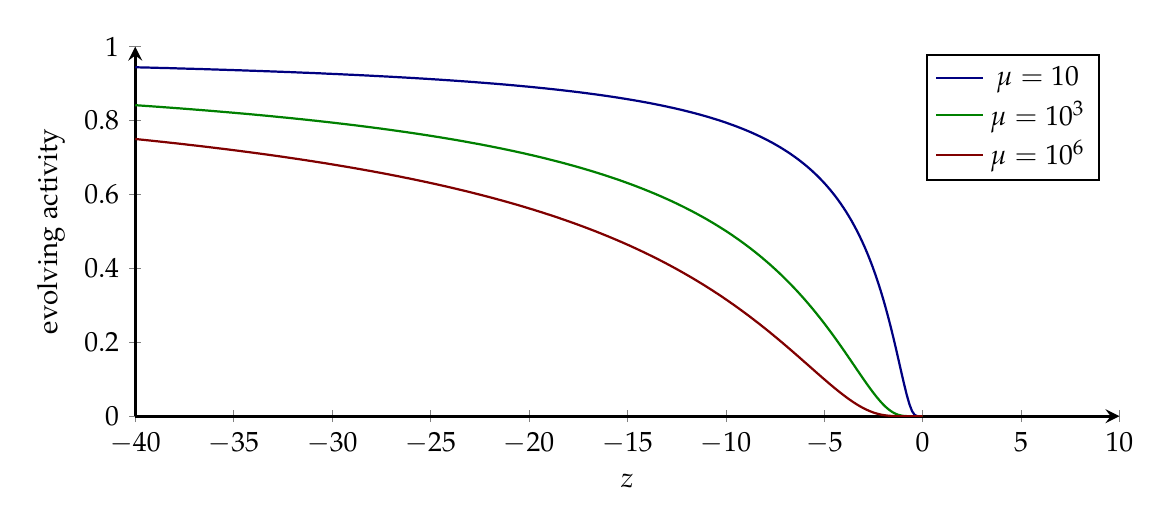
\begin{tikzpicture} \begin{axis}[ 
	thick,
	width=0.6\textwidth,
	x=1cm/4,
	xmax=10, ymax=1,
	axis line style=very thick,
	axis x line=bottom,
	axis y line=left,
	xlabel={$z$},
	ylabel={evolving activity},
] 
	\addplot[color=blue!50!black,samples=300,domain=-40:-0.001] {exp(ln(10)*(1/x))}; 
	\addplot[color=green!50!black,samples=300,domain=-40:-0.001] {exp(ln(1000)*(1/x))}; 
	\addplot[color=red!50!black,samples=300,domain=-40:-0.001]
	{exp(ln(100000)*(1/x))}; 
	\legend{$\mu=10$,$\mu=10^3$,$\mu=10^6$};
	\end{axis} \end{tikzpicture} 
\end{center}

\begin{theorem}
Evolving activity satisfies both normalization and initialization.
\end{theorem}
\begin{proof}
Since the initial value of $z$ is $0$ and $z\leq 0$, by definition we have
$a(G_t,v)=0$ if $v$ is never changed, because there are no chance for $z$
to be less than $0$.

Since $\mu>1$, and $z\in\mathbb{R}$, we have $0<a(G_t,v)<1$.
\end{proof}

\begin{theorem}
Evolving activity satisfies monotonicity.
\end{theorem}
\begin{proof}
Refer to \eqref{eq-mono}, we have $z$ for $G$ at time $t$ is decreased, and
is thus at least $\eta w$ less than $z'$ for $G'$ at time $t$, namely
\begin{equation}z\leq z'-\eta w<0.\end{equation}
If $z'=0$, then
\begin{equation}
a(G'_t,v)=0<a(G_t,v)=\mu^{1/z}.
\end{equation}
Otherwise if $z'<0$,
\begin{equation}
z<z'\implies \mu^{1/z}>\mu^{1/z'},
\end{equation}
hence
\begin{equation}
a(G_t,v)>a(G'_t,v).
\end{equation}
\end{proof}

\begin{theorem}
Evolving activity satisfies symmetry.
\end{theorem}
\begin{proof}
Refer to \eqref{eq-sym}, we can write
\begin{equation}
g(a(G_t,v),n,\left\{w_i\right\},\varepsilon)=\begin{cases}
0 &(z^*\geq 0)\\
\mu^{1/z^*}& (z^*=0)
\end{cases},
\end{equation}
where
\begin{equation}
z^*=z+\varepsilon-\eta \sum_i w_i,
\end{equation}
and
\begin{equation}
z=\begin{cases}
0&(a(G_t,v)=0)\\
1/\log_{\mu}a(G_t,v)&(a(G_t,v)>0)
\end{cases}.
\end{equation}
So such $g$ exists.
\end{proof}

\begin{theorem}
Evolving activity satisfies locality.
\end{theorem}
\begin{proof}
By definition, $z$ will not be affected by non-local change.
\end{proof}

\begin{theorem}
Evolving activity satisfies integrity.
\end{theorem}
\begin{proof}
First we consider the base case, where we add edges to the vertex $v$ at time $t_i$ and $z=0$ initially. 

Denote the sum of weights of these new edges by $w(t_i)$, so $z$ decreases to
$-\eta w(t_i)$ from 0. By the definition of $z$, we write $z$ as the function
of $t$, which is $z(t)=t-t_i-\eta w(t_i)$. For simplify we choose $\mu=e$ here,
it's similar to prove for other values of $\mu$. Now the integrity is as
follows:

\begin{equation}
\begin{split}
\int_{t_i}^{t_i+\eta w(t_i)} a(G_t,v) \mathrm{d}t &= \int_{t_i}^{t_i+\eta
w(t_i)} e^{\frac{1}{t-t_i-\eta w(t_i)}} \mathrm{d}t \\
&= \int_{-\eta w(t_i)}^{0} e^{\frac{1}{t}} \mathrm{d}t.
\end{split}
\end{equation}

Notice that $e^{1/t}<1(t<0)$, so it's easy for this direction
\begin{equation}
\int_{-\eta w(t_i)}^{0} e^{\frac{1}{t}} \mathrm{d}t< \eta w(t_i).
\end{equation}

Define $f(x)=\int_{-x}^{0} e^{1/t} \mathrm{d}t - \frac{x}{10}$, from
$f'(x)=e^{-1/x}-\frac{1}{10}$, at least we can see $f(x)$ increases when $x\ge
1$. So $f(x)\ge f(1)\approx 0.05>0$.

Now we have the other direction: 
\begin{equation}
\int_{-\eta w(t_i)}^{0} e^{\frac{1}{t}} \mathrm{d}t>\frac{\eta w(t_i)}{10},
\end{equation}
as long as $\eta w(t_i)\ge 1$.

Next we return to a general case. 

We show the theorem holds for each "phase", where we call the period of time
when $z<0$ a "phase" and a "phase" starts and ends both with $z=0$. Consider a
"phase" starting from $t_i$ and ending at $t_j$, some edges whose sum of
weights is $w(t_k)$ are added to $v$ at time $t_k(i\le k\le j)$, so $z$
decreases from $z(t_k)$ to $z(t_k)-\eta w(t_k)$ sharply.

One can verify that
\begin{equation}
\int_{t_i}^{t_j} a(G_t,v) \mathrm{d}t< \eta \sum_{k=i}^j w(t_k),
\end{equation}
easily since we still have $\mu^{1/z(t)}<1$.

As for the other direction, notice that at time $t_{k+1}$, there are two cases.
One is that $z(t_{k+1})$ has increased equal or above $z(t_k)$, namely we can
find some $t_k^*\in (t_k, t_{k+1})$, where $t_k^*$ is defined to satisfy that
$z(t_k)=z(t_k^*)$ for all $k$. So we have \begin{equation}
\int_{t_k}^{t_{k+1}} \mu^{\frac{1}{z(t)}} \mathrm{d}t \ge \int_{t_k}^{t_k^*}
\mu^{\frac{1}{z(t_k)+t-t_k}} - \mu^{\frac{1}{z(t_{k})}}\mathrm{d}t.
\end{equation}
The other case is that $z(t_{k+1})$ is still less than $z(t_{k})$, in other
words, we will find $t_k^*>t_{k+1}$.  

Now from
\begin{equation}
z(t)=
\begin{cases}
z(t_k)+t-t_k&  t\in (t_k, t_{k+1})\\
z(t_{k+1})+t-t_{k+1}& t\in (t_{k+1}, t_{k+2}),
\end{cases}
\end{equation}
we have:
\begin{equation}
\begin{split}
&\int_{t_k}^{t_{k+2}} \mu^{\frac{1}{z(t)}} \mathrm{d}t\\
\ge{}& \int_{t_k}^{t_{k+1}^*} \mu^{\frac{1}{z(t)}} \mathrm{d}t \\
={}&\int_{t_k}^{t_{k+1}} \mu^{\frac{1}{z(t_k)+t-t_k}} - \mu^{\frac{1}{z(t_{k})}}
\mathrm{d}t+ \int_{t_{k+1}}^{t_{k+1}^*} \mu^{\frac{1}{z(t_{k+1})+t-t_{k+1}}}\\& -
\mu^{\frac{1}{z(t_{k+1})}} \mathrm{d}t + (t_{k+1}^*-t_{k+1})\mu^{\frac{1}{z(t_{k+1})}}\\
\ge{}& \int_{t_k}^{t_{k}^*} \mu^{\frac{1}{z(t_k)+t-t_k}} -
\mu^{\frac{1}{z(t_{k})}}\mathrm{d}t + \int_{t_{k+1}}^{t_{k+1}^*}
\mu^{\frac{1}{z(t_{k+1})+t-t_{k+1}}} - \mu^{\frac{1}{z(t_{k+1})}}\mathrm{d}t,
\end{split}
\end{equation}
by an easy induction, one can split a "phase" into integrals in the form 
\begin{equation}
\int_{t_k}^{t_{k}^*} \mu^{\frac{1}{z(t_k)+t-t_k}} - \mu^{\frac{1}{z(t_{k})}}\mathrm{d}t
\end{equation}
 Since $ \mu^{1/z}$ decreases as $z$ becomes larger, we can reduce it to the base case now.

Above all, the theorem holds.
\end{proof}



\begin{definition}[Evolving Centrality]
\textbf{Evolving centrality} $\textbf{x}(G_t)$ is a vector in space
$\mathbb{R}^{|V|}$, where
\begin{equation}
\mathbf{x}=\alpha DLA^\bullet \mathbf{x} + \beta\mathbf{1},
\end{equation}
$A^\bullet$ is the 0/1 adjacency matrix of $E^\bullet_t$ as defined in section 2,
because centrality accentuate more on the structure of the network but not the
intensity of edges. And
$D,L$ are diagonal matrices such that
\begin{equation}
D_{ij}=\begin{cases}
0&(i\neq j)\\
\mathit{Act}(G_t,v_i)&(i=j)
\end{cases}\qquad
L_{ij}=\begin{cases}
0&(i\neq j)\\
1/k^\bullet(G_t,v_i)&(i=j)
\end{cases}.
\end{equation}
Then $\textbf{x}_i(G_t)$ is the centrality for node $v_i$ in $G_t$, and is
scale-relative to the influence of $v_i$ in the network at time $t$.
\end{definition}

The equivalent form of evolving centrality $x(G_t,v_i)$ is 
\begin{equation}
x_i(G_t,v_i)=\alpha\sum_j\frac{A^\bullet_{ij}
\mathit{Act}(G_t,v_j)x_j(G_t,v_j)}{k^\bullet(G_t,v_j)}+\beta.
\end{equation}

We can also change the model into a directional graph, and study the network as
a citation network:

\begin{definition}[Evolving PageRank]
\textbf{Evolving PageRank} $\textbf{x}(G_t)$ is a vector in space
$\mathbb{R}^{|V|}$, where
\begin{equation}
\mathbf{x}=\alpha DLA \mathbf{x} + \beta\mathbf{1},
\end{equation}
where $A_{ij}$ stands for the total weight of edges from $j$ to $i$,
\begin{equation}
D_{ij}=\begin{cases}
0&(i\neq j)\\
\mathit{Act}(G_t,v_i)&(i=j)
\end{cases};\qquad
L_{ij}=\begin{cases}
0&(i\neq j)\\
1/k_{\mathrm{out}}(G_t,v_i)&(i=j)
\end{cases}.
\end{equation}
\end{definition}

The equivalent form of evolving PageRank $x(G_t,v_i)$ is 
\begin{equation}
x_i(G_t,v_i)=\alpha\sum_j
\frac{A_{ij}\mathit{Act}(G_t,v_j)x_j(G_t,v_j)}{k_{\mathrm{out}}(G_t,v_j)}
+\beta.
\end{equation}

\section{Data structure and Algorithms}
\subsection{Maintaining the graph}
We formally define the abstract data type for the pure growing model, and
create algorithmic functions to the data structure.

A evolving network $G_t(V,E_t)$ is stored in following contents:
\begin{itemize}
\item \textit{currentTime}, a non-negative real number.
\item $\mu$, a real number in range $(1,+\infty)$.
\item $\eta$, a non-negative real number.
\item \textit{edgeList}[$1\dots|V|$], an array that every of
whose entry points to a sorted array again, consisting the description of the
in edges of $v_i$ in the graph, each with elements:
\begin{itemize}
\item $u$, the other end point of the edge.
\item $t$, the time when this edge is added. (the array is sorted by $t$)
\item $w$, the weight of the edge, can be reduced if the network is
unweighted.
\item $s$, the sum of all previous $w$, including this one.
\item $z$, the status variable for calculating the evolving activity of node
$v_i$ at time $t$ after updating this edge.
\end{itemize}

\item \textit{edgeListReduced}[$1\dots|V|$], an array that every of
whose entry points to a sorted array again, consisting the description of the
neighbors of $v_i$ in the graph, each with a element $u$ (sorted by $u$).

\item \textit{father}[$1\dots|V|$], an array exploited by the historical
union-find algorithm\cite{tarjan1975efficiency} (a weakened model), which
will be discussed later. Each of the elements contains:
\begin{itemize}
\item $u$, the identity of $v_i$'s father node if $u>0$, otherwise $v_i$
is a root node, and $(-u)$ is the size of the tree.
\item $t$, the time when $u$ becomes non-zero.
\end{itemize}

\end{itemize}
\textbf{Space complexity:} $O(|V|+|E|)$.

The data type contains following functions:
\begin{itemize}
\item \textsc{Add Edge}($v_i,v_j,t,w$)

Add $e(v_i,v_j,t,w)$ to the graph and update the graph,
defined in algorithm \ref{alg-add}.
\item \textsc{Query Degree}($t,v$)

Return $k(G_t,v)$, defined in algorithm \ref{alg-deg}.
\item \textsc{Query Connectivity}($t,u,v$)

Return whether $u$ and $v$ is connected in the network at time $t$, defined in
algorithm \ref{alg-con}.

\item \textsc{Query Activity}($t,v$)

Returns the evolving activity $a_{\mu,\eta}(G_t,v)$, defined in algorithm
\ref{alg-act}.

\item \textsc{Query Centrality}($t$, $\alpha$, $\beta$, $\mathbf{x}_0$, $m$)

Return the active centrality vector $\mathbf{x}(G_t)$. Algorithm \ref{alg-cen}
use the iteration method start with $\mathbf{x}_0$ and for $m$ times.

\item \textsc{Modify Mu}($\mu'$)

Change the value of $\mu$ which defines the evolving activity, in case the
current $\mu$ is inappropriate, defined in algorithm \ref{alg-mu}.

\item \textsc{Modify Eta}($\eta'$)

Change the value of $\eta$ which defines the evolving activity, in case the
current $\eta$ is inappropriate, defined in algorithm \ref{alg-eta}.
\end{itemize}

\begin{algorithm}[htbp]
\caption{\textsc{Add Edge}($v_i,v_j,t,w$)}
\label{alg-add}
\textbf{Time Complexity:} $O(\log |V|)$\\
\textbf{Additional Space:} $O(1)$
\begin{algorithmic}[1]
\Require $1\leq i,j\leq |V|$ and $t\geq \mathit{currentTime}$ and $w>0$.
\Ensure $G_t$ is up-to-date.
\State $\mathit{currentTime}\gets t$;
\State $z_1\gets\mathit{edgeList}[i].\mathrm{lastElement}.z$;
\State $t_1\gets\mathit{edgeList}[i].\mathrm{lastElement}.t$;
\State $s_1\gets\mathit{edgeList}[i].\mathrm{lastElement}.s$;
\State $z_1\gets z_1+\mathit{currentTime}-t_1$;
\If {$z_1>0$} \State $z_1\gets 0$;\EndIf
\State $z_1\gets z_1-\eta\cdot w$;
\State $z_2\gets\mathit{edgeList}[j].\mathrm{lastElement}.z$;
\State $t_2\gets\mathit{edgeList}[j].\mathrm{lastElement}.t$;
\State $s_2\gets\mathit{edgeList}[j].\mathrm{lastElement}.s$;
\State $z_2\gets z_2+\mathit{currentTime}-t_2$;
\If {$z_2>0$} \State $z_2\gets 0$;\EndIf
\State $z_2\gets z_2-\eta\cdot w$;
\State append ($j$, $t$, $w$, $s_2+w$, $z_2$) to \textit{edgeList}[$i$];
\State append ($i$, $t$, $w$, $s_1+w$, $z_1$) to \textit{edgeList}[$j$];
\If{ binary search on \textit{edgeListReduced}[$i$] did not find $j$}
\State insert $j$ to \textit{edgeListReduced}[$i$] in appropriate position;
\State binary search $i$ on \textit{edgeListReduced}[$j$];
\State insert $i$ to \textit{edgeListReduced}[$j$] in appropriate position;
\EndIf
\State $p\gets \Call{Find Root}{i,\mathit{currentTime}}$;
\State $q\gets \Call{Find Root}{j,\mathit{currentTime}}$;
\If{$p\neq q$}
\State \Call{Merge}{$p$,$q$}
\EndIf
\end{algorithmic}
\end{algorithm}

\begin{algorithm}[htbp]
\caption{\textsc{Find Root}($i$, $t$)}\label{alg-find}
\textbf{Time Complexity:} $O(\log |V|)$\\
\textbf{Additional Space:} $O(1)$
\begin{algorithmic}[1]
\Require $1\leq i\leq |V|$
\Ensure return the root of the union tree containing $v_i$ at time $t$.
\State $\mathit{currentTime}\gets t$;
\If {$\mathit{father}[i].u>0$ and $\mathit{father}[i].t\leq t$}
	\State \Return{\Call{FindRoot}{$\mathit{father}[i].u$, $t$}};
\Else
	\State \Return{$i$};
\EndIf
\end{algorithmic}
\end{algorithm}

\begin{algorithm}[htbp]
\caption{\textsc{Merge}($p$,$q$)}
\label{alg-merge}
\textbf{Time Complexity:} $O(1)$\\
\textbf{Additional Space:} $O(1)$
\begin{algorithmic}[1]
\Require $\mathit{father}[p].u<0$ and $\mathit{father}[q].u<0$
and $p\neq q$.
\Ensure Union trees $p$ and $q$.
\State $x \gets -\mathit{father}[p].u$;
\State $y \gets -\mathit{father}[q].u$;
\If {$x>y$}
	\State $\mathit{father}[q].u\gets p$;
	\State $\mathit{father}[q].t\gets \mathit{currentTime}$;
	\State $\mathit{father}[p].u \gets \mathit{father}[p].u-y$;
\Else
	\State $\mathit{father}[p].u\gets q$;
	\State $\mathit{father}[p].t\gets \mathit{currentTime}$;
	\State $\mathit{father}[q].u\gets \mathit{father}[q].u-x$;
\EndIf
\end{algorithmic}
\end{algorithm}

\begin{algorithm}[htbp]
\caption{\textsc{Query Connectivity}($t$,$p$,$q$)}
\label{alg-con}
\textbf{Time Complexity:} $O(\log |V|)$\\
\textbf{Additional Space:} $O(1)$
\begin{algorithmic}[1]
\Require $1\leq p,q \leq |V|$.
\Ensure return whether $p$ and $q$ are connected at time $t$.
\State \Return{$\Call{Find Root}{p,t}=\Call{Find Root}{q,t}$};
\end{algorithmic}
\end{algorithm}

\begin{algorithm}[htbp]
\caption{\textsc{Query Degree}($t$,$v_i$)}
\label{alg-deg}
\textbf{Time Complexity:} $O(\log |V|)$\\
\textbf{Additional Space:} $O(1)$
\begin{algorithmic}[1]
\Require $1\leq i\leq |V|$.
\Ensure return the degree of $v_i$ at time $t$.
\State $p\gets\text{binary search }\mathit{edgeList}[i]\text{ for
the latest edge before }t$;
\If{ $p$ not found}
\State\Return{$0$}
\Else
\State \Return{$p.s$};
\EndIf
\end{algorithmic}
\end{algorithm}


\begin{algorithm}[htbp]
\caption{\textsc{Query Activity}($t$,$v_i$)}
\label{alg-act}
\textbf{Time Complexity:} $O(\log |V|)$\\
\textbf{Additional Space:} $O(1)$
\begin{algorithmic}[1]
\Require $1\leq i\leq |V|$.
\Ensure return the evolving activity $a_{\mu,\eta}(G_t,v_i)$.
\State $p\gets\text{binary search }\mathit{edgeList}[i]\text{ for
the latest edge before }t$;
\If{ $p$ not found}
\State\Return{$0$}
\Else
\State $z=\min(p.z+t-p.t,0)$;
\If{$z=0$}
\State \Return{$0$};
\Else
\State \Return{$\mu^{1/z}$};
\EndIf
\EndIf
\end{algorithmic}
\end{algorithm}

\begin{algorithm}[htbp]
\caption{\textsc{Modify Mu}($\mu'$)}
\label{alg-mu}
\textbf{Time Complexity:} $O(1)$\\
\textbf{Additional Space:} $O(1)$
\begin{algorithmic}[1]
\State $\mu\gets\mu'$;
\end{algorithmic}
\end{algorithm}

\begin{algorithm}[htbp]
\caption{\textsc{Modify Eta}($\eta'$)}
\label{alg-eta}
\textbf{Time Complexity:} $O(1)$\\
\textbf{Additional Space:} $O(1)$
\begin{algorithmic}[1]
\State $\eta\gets\eta'$;\State\Comment{Incompatible with historical queries.
The alternative is to rebuild the whole graph.}
\end{algorithmic}
\end{algorithm}


\begin{algorithm}[htbp]
\caption{\textsc{Query Centrality}($t$,$\alpha$,$\beta$,
$\mathbf{x}_0$,$m$)}
\label{alg-cen}
\textbf{Time Complexity:} $O(mK|V|)$, $K$ is the sparsity constant.\\
\textbf{Additional Space:} $O(|V|)$
\begin{algorithmic}[1]
\Require $0<\alpha<\lambda_1(A^\bullet(G_t))^{-1}$ and $\beta>0$ and $m>0$. Here
$\lambda_1(A)$ is the maximal positive eigenvalue of matrix $A$.
\Ensure return the active centrality $\mathbf{x}(G_t)$.
\For{$i\gets 1\dots|V|$}
\State $a[i]\gets \Call{Query Activity}{t,v_i}$;
\State $k[i]\gets \mathrm{size}(\mathit{edgeListReduced}[i])$;
\State $\mathbf{x}[i]\gets \mathbf{x}_0[i]$;
\EndFor
\For{$\mathit{count}\gets 1\dots m$}
\For{$i\gets 1\dots|V|$}
\State $\mathbf{x'}[i]\gets \beta$;
\EndFor
\For{$i\gets 1\dots|V|$}
\ForAll{$j\in\mathit{edgeListReduced}[i]$}
\State $\mathbf{x'}[i]\gets \mathbf{x'}[i]+\alpha\cdot
a[j]\cdot\mathbf{x}[j]/k[j]$
\EndFor\EndFor
\For{$i\gets 1\dots|V|$}
\State $\mathbf{x}[i]\gets \mathbf{x'}[i]$;
\EndFor
\EndFor
\State\Return{$\mathbf{x}$};
\end{algorithmic}
\end{algorithm}

\subsection{Optimization and Parallelization}
In most cases, we only need to query the latest properties of the graph, i.e.,
$t=\mathit{currentTime}$. And we observe that in algorithm \ref{alg-con},
\ref{alg-deg} and \ref{alg-act}, the binary search can be replace by simply find
the last entry of the argument sequence. So those three algorithms can be done
in $O(1)$ time if we do not perform historical queries.

What the core part of algorithm \ref{alg-cen} does is only the multiplication
of a sparse matrix to a vector, which is a classical problem called sparse
matrix-vector multiplication (SpMV). This problem can be easily solve in both
throughput-oriented and latency-oriented processors in
parallel\cite{williams2009optimization, bell2008efficient,
bell2009implementing, catalyurek1999hypergraph, zhuo2005sparse}.  This is a
good news to us because nowadays parallel machine is much more common in
companies, research facilities and even with desktop computers, thanks to the
emergence of GPGPU platforms such as CUDA and OpenCL.

\section{Experiment}
\subsection{Data Generation} 
Our data generation is base on real social networks provided by \cite{database1,
database2}. Unfortunately, those databases do not contain evolving history
recorded data, so we simulate the evolving history by use the
authentic graph as the final state of the tested dynamic graph.
We give a random permutation to the edges, in a way such that:
\begin{itemize}
\item There will always
be just one component -- known as the giant component. We never add an edge out
of the giant component, so the evolving of the network seems to have increasing
vertices joining to the network.
\item The time delay of two adjacent new edges is inversely proportional to the
size of the giant component. So the average activity of any individual node
would not change tremendously.
\end{itemize}
Because the final state
is from real world data, it is ensured 
the evolving graph generated by our model will satisfy all the property that we
discussed in section 2.2. In addition, Kumar introduced how to generate
an artificial evolving social networks\cite{kumar2010structure}.

\subsection{Program}
We have implemented the algorithms using C++ language without compiler
optimization, and all executions are done under a typical PC with 
Intel (R) Core (TM) i3 CPU M380  @ 2.53GHz, 2GB RAM.
	
The program maintains a dynamic graph which contains $n$ vertices and does not
have any edge at the beginning.
It support the following operations:
\begin{itemize}
	\item \textsc{Add Edge$(u,v,w)$:} increase the time counter by one, and then add an edge
		of weight $w$ between vertex $u$ and vertex $v$.
	\item \textsc{Query Degree$(t,u)$:} ask for the degree of $u$ at time $t$.
	\item \textsc{Query Activity$(t,u)$:} ask for the activity (as we defined) of $u$ at time $t$.
	\item \textsc{Query Connectivity$(t,u,v)$:} ask that whether vertices $u,v$ is connected or not
		$u$ at time $t$.
\end{itemize}
Note that the time counter is initially zero.
Each operation cost $O(\log n)$ time in our implemented algorithm.

\subsubsection{Checking for Correctness}
We implemented a simple algorithm together which cost $O(\max\{n,m\})$ time for
each operation, where $m$ is the number of edges before the operation.  We have
generated several small test cases and compare the results between the simple
program and our $O(\log n)$ program.  There is no difference found between
outputs of the two programs.

\subsubsection{Checking for Time Complexity}
We have generated several huge test cases to test the running time of the program.
The following plots shows the informations about the cases and the running results.

\begin{center} 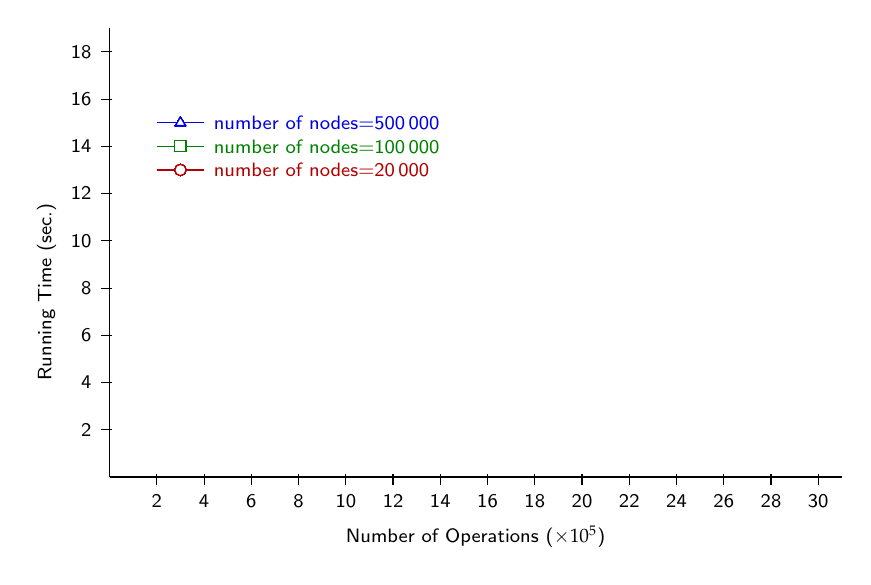
\begin{tikzpicture}[y=.3cm, x=.3cm, font=\sffamily]
 	%axis
	\draw (0,0) -- coordinate (x axis mid) (31, 0);
	\draw (0,0) -- coordinate (y axis mid) (0, 19);
	%ticks
	\foreach \x in {2,4,...,30}
		\draw (\x,1pt) -- (\x,-3pt) node[anchor=north] {\scriptsize \x};
	\foreach \y in {2,4,...,18}
		\draw (1pt,\y) -- (-3pt,\y) node[anchor=east] {\scriptsize \y};
	%labels      
	\node[below=0.5cm] at (x axis mid) {\scriptsize Number of Operations ($\times10^5$)};
	\node[rotate=90, left=0.8cm] at (0, 12) {\scriptsize Running Time (sec.)};
	%plots
	\draw[color=red!70!black] plot[mark=*, mark options={fill=white}] file {exp-n2w};
	\draw[color=green!50!black] plot[mark=square*, mark options={fill=white}] file {exp-n10w};
	\draw[color=blue!80!black] plot[mark=triangle*, mark options={fill=white}] file {exp-n50w};
	%legend
	\begin{scope}[shift={(2,13)}]
	\draw[color=red!70!black] (0,0) -- plot[mark=*, mark options={fill=white}] (1,0) -- (2,0)
		node[right]{\scriptsize number of nodes=20\,000};
	\draw[color=green!50!black] (0,1) -- plot[mark=square*, mark options={fill=white}] (1,1) -- (2,1)
		node[right]{\scriptsize number of nodes=100\,000};
	\draw[color=blue!90!black] (0,2) -- plot[mark=triangle*, mark options={fill=white}] (1,2) -- (2,2)
		node[right]{\scriptsize number of nodes=500\,000};
	\end{scope}
\end{tikzpicture} \end{center}

We can verify that our algorithm model works efficiently with those four kinds
of basic operations.

\begin{center} 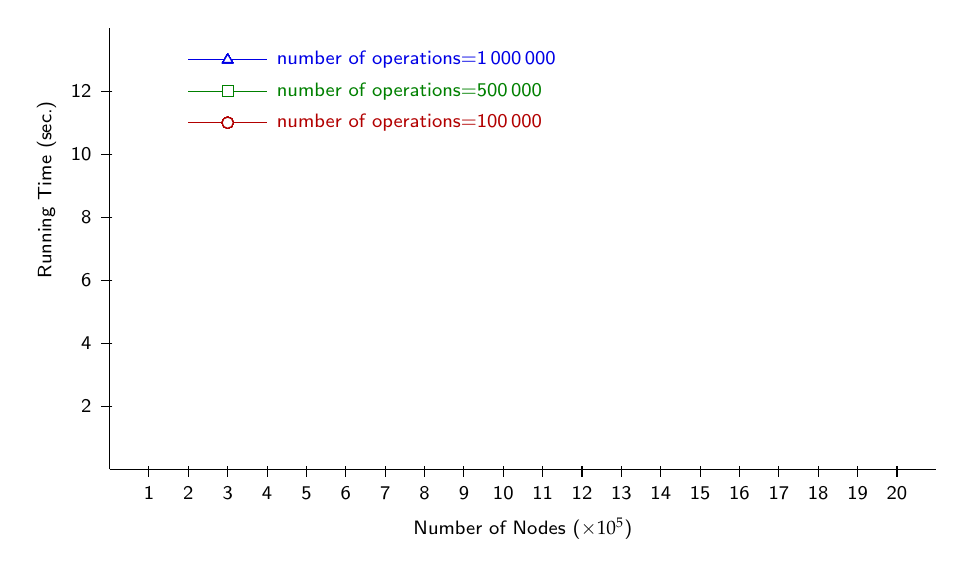
\begin{tikzpicture}[y=.4cm, x=.5cm, font=\sffamily]
 	%axis
	\draw (0,0) -- coordinate (x axis mid) (21, 0);
	\draw (0,0) -- coordinate (y axis mid) (0, 14);
	%ticks
	\foreach \x in {1,2,...,20}
		\draw (\x,1pt) -- (\x,-3pt) node[anchor=north] {\scriptsize \x};
	\foreach \y in {2,4,...,13}
		\draw (1pt,\y) -- (-3pt,\y) node[anchor=east] {\scriptsize \y};
	%labels      
	\node[below=0.5cm] at (x axis mid) {\scriptsize Number of Nodes ($\times10^5$)};
	\node[rotate=90, left=0.8cm] at (0, 12) {\scriptsize Running Time (sec.)};
	%plots
	\draw[color=red!70!black] plot[mark=*, mark options={fill=white}] file {exp-q10w};
	\draw[color=green!50!black] plot[mark=square*, mark options={fill=white}] file {exp-q50w};
	\draw[color=blue!80!black] plot[mark=triangle*, mark options={fill=white}] file {exp-q100w};
	%legend
	\begin{scope}[shift={(2,11)}]
	\draw[color=red!70!black] (0,0) -- plot[mark=*, mark options={fill=white}] (1,0) -- (2,0)
		node[right]{\scriptsize number of operations=100\,000};
	\draw[color=green!50!black] (0,1) -- plot[mark=square*, mark options={fill=white}] (1,1) -- (2,1)
		node[right]{\scriptsize number of operations=500\,000};
	\draw[color=blue!90!black] (0,2) -- plot[mark=triangle*, mark options={fill=white}] (1,2) -- (2,2)
		node[right]{\scriptsize number of operations=1\,000\,000};
	\end{scope}
\end{tikzpicture} \end{center}

The time efficiency in terms of $|V|$ proves to have logarithm growth as
expected.

\subsection{Centrality Analysis}
Here are some traces of both the evolving centrality and the classical PageRank
centrality of specific nodes.

We generates evolving network data in the same model discussed above, with
$|V|\leq 6\,000$ and $|E|\leq 30\,000$. All iterations run for enough time,
until the maximum magnitude of change in individual centralities (known as the
$\infty$-norm of $\Delta\mathbf{x}$) is smaller than $10^{-4}$ by absolute value.
We also calculate the static PageRank centrality in parallel, which do not have
the activity metric as coefficients. All of our calculation assumes
$\alpha=0.8$, and $\beta=1$.

\begin{itemize}
\item The centrality trace graph for some representative node, when $\mu=4096$ and
$\eta=1000$:
\begin{center} \begin{tikzpicture}[y=.4cm, x=.5cm, font=\sffamily]
	\draw (0,0) -- coordinate (x axis mid) (21, 0);
	\draw (0,0) -- coordinate (y axis mid) (0, 11);
	\node[below=0.5cm] at (x axis mid) {\scriptsize Time ($\times10^3$)};
	\node[rotate=90, left=0.8cm] at (0, 10) {\scriptsize Magnitude of
	Centrality};
	\foreach \x in {1,2,...,20}
	\draw (\x,1pt) -- (\x,-3pt) node[anchor=north] {\scriptsize \x};
		\foreach \y in {1,2,...,11}
		\draw (1pt,\y) -- (-3pt,\y) node[anchor=east] {\scriptsize \y};
	\draw[color=red!70!black,line width=1pt] plot file {exp-g3-1};
	\draw[color=blue!70!black] plot file {exp-g3-2};
	\begin{scope}[shift={(2,8)}]
	\draw[color=red!70!black,line width=1pt] (0,0) -- (2,0)
		node[right]{\scriptsize evolving centrality};
	\draw[color=blue!50!black] (0,1) -- (2,1)
		node[right]{\scriptsize static centrality};
	\end{scope}
\end{tikzpicture} \end{center}
Evolving centrality is smaller then static one, because we applied the
activity coefficients which is less than $1$. The overall tendency of those
traces are similar, but the evolving centrality declines more quickly.
\begin{center} \begin{tikzpicture}[y=.4cm, x=.5cm, font=\sffamily]
	\draw (0,0) -- coordinate (x axis mid) (21, 0);
	\draw (0,0) -- coordinate (y axis mid) (0, 11);
	\node[below=0.5cm] at (x axis mid) {\scriptsize Time ($\times10^3$)};
	\node[rotate=90, left=0.8cm] at (0, 10) {\scriptsize Magnitude of
	Centrality};
	\foreach \x in {1,2,...,20}
	\draw (\x,1pt) -- (\x,-3pt) node[anchor=north] {\scriptsize \x};
		\foreach \y in {1,2,...,11}
		\draw (1pt,\y) -- (-3pt,\y) node[anchor=east] {\scriptsize \y};
	\draw[color=red!70!black,line width=1pt] plot file {exp-g9-1};
	\draw[color=blue!70!black] plot file {exp-g9-2};
	\begin{scope}[shift={(2,8)}]
	\draw[color=red!70!black,line width=1pt] (0,0) -- (2,0)
		node[right]{\scriptsize evolving centrality};
	\draw[color=blue!50!black] (0,1) -- (2,1)
		node[right]{\scriptsize static centrality};
	\end{scope}
\end{tikzpicture} \end{center}
We can observe that two centralities can react quite differently to changes.

\item The centrality trace graph for some representative node, when $\mu=2^{20}$ and
$\eta=2000$:
\begin{center} \begin{tikzpicture}[y=.4cm, x=.5cm, font=\sffamily]
	\draw (0,0) -- coordinate (x axis mid) (21, 0);
	\draw (0,0) -- coordinate (y axis mid) (0, 11);
	\node[below=0.5cm] at (x axis mid) {\scriptsize Time ($\times10^3$)};
	\node[rotate=90, left=0.8cm] at (0, 10) {\scriptsize Magnitude of
	Centrality};
	\foreach \x in {1,2,...,20}
	\draw (\x,1pt) -- (\x,-3pt) node[anchor=north] {\scriptsize \x};
		\foreach \y in {1,2,...,11}
		\draw (1pt,\y) -- (-3pt,\y) node[anchor=east] {\scriptsize \y};
	\draw[color=red!70!black,line width=1pt] plot file {exp-g8-1};
	\draw[color=blue!70!black] plot file {exp-g8-2};
	\begin{scope}[shift={(2,8)}]
	\draw[color=red!70!black,line width=1pt] (0,0) -- (2,0)
		node[right]{\scriptsize evolving centrality};
	\draw[color=blue!50!black] (0,1) -- (2,1)
		node[right]{\scriptsize static centrality};
	\end{scope}
\end{tikzpicture} \end{center}
By elongating the activity delay, the declination becomes slower for evolving
centrality. However, it still declines faster than the static one.
\begin{center} \begin{tikzpicture}[y=.4cm, x=.5cm, font=\sffamily]
	\draw (0,0) -- coordinate (x axis mid) (21, 0);
	\draw (0,0) -- coordinate (y axis mid) (0, 11);
	\node[below=0.5cm] at (x axis mid) {\scriptsize Time ($\times10^3$)};
	\node[rotate=90, left=0.8cm] at (0, 10) {\scriptsize Magnitude of
	Centrality};
	\foreach \x in {1,2,...,20}
	\draw (\x,1pt) -- (\x,-3pt) node[anchor=north] {\scriptsize \x};
		\foreach \y in {1,2,...,11}
		\draw (1pt,\y) -- (-3pt,\y) node[anchor=east] {\scriptsize \y};
	\draw[color=red!70!black,line width=1pt] plot file {exp-g11-1};
	\draw[color=blue!70!black] plot file {exp-g11-2};
	\begin{scope}[shift={(2,8)}]
	\draw[color=red!70!black,line width=1pt] (0,0) -- (2,0)
		node[right]{\scriptsize evolving centrality};
	\draw[color=blue!50!black] (0,1) -- (2,1)
		node[right]{\scriptsize static centrality};
	\end{scope}
\end{tikzpicture} \end{center}
We observe a clear concave in evolving centrality from time $12\,000$ to
$16\,000$. Perhaps the reason for that is the neighbors of the vertex becomes
less active, despite the static structural centrality is high.
\end{itemize}

\section{Conclusion and Perspective}
So far, we have established and verified the framework for analysing an
evolving social network. We defined two metrics for the networks, namely
\textbf{evolving activity} and \textbf{evolving centrality}. The
experiment showed that our model can successful compute both of the metrics in
practical cases.

By the final experiment, we can observe that the increase on magnitude of
evolving centrality is similar to that of the static one. However, when the
influence of a node stops increase so fast, our evolving centrality quickly
pulls back, while the static centrality usually keeps a high value for long
time. In many fields, the social concern are supposed to be sensitive to time
, innovation and activeness, instead of imposing more attention to historical
issues that are once very popular. Those fields such as web-page search
engine, ranking of movie actors, seeking hot scholar topics, etc.
By using evolving centrality, the increment of actions of a node and its
closely related region will be more notable in increment of its ranking of
influence, whereas the static centrality is more likely to trigger
conformity on social preference\cite{cialdini2004social} because people will
have less chance to see and rate new information, which may prevent high
quality information from getting popular, and even worse, hasten the
monopolization in the commercial
aspect.

The evolving centrality is more sensitive to activities of the surroundings, so
it usually changes more dramatically than static centrality which is more
stable. Dynamic metrics provides new methods for network analysis.


\bibliography{paper}
\end{document}

% vim: set ts=8 sw=8 noet sts=8 tw=79 indentexpr= fdm=marker foldmarker=<<<,>>>:
